\smartsection{Foundation \& Security}
\label{sec:foundation-security}

\smartsubsection{Overview}

Before any application-level component of the Smart Surveillance System was
built, a security baseline was established across both machines in the
deployment: the Orange Pi Zero Plus 2 board and the laptop acting as the
development/MQTT-broker host. This baseline is a hard requirement of the
assignment and underpins the security experiments of the original task
sheet (numbered \textbf{3-6} and \textbf{3-7}), so it was completed first
and never revisited.

Four controls were put in place:
\begin{itemize}
    \item \keyterm{SSH hardening} — root login disabled unconditionally,
    with a choice between key-based or password authentication.
    \item \keyterm{MQTT authentication} — the Mosquitto broker rejects
    anonymous connections; a dedicated, credentialed client account is
    required.
    \item \keyterm{TLS certificate provisioning} — a self-signed
    certificate is generated with its Common Name (CN) set to the
    student ID, as required for the HTTPS work in
    Section~\ref{sec:image-processing} onward.
    \item \keyterm{Secrets management} — no password, API key, or
    certificate ever appears hardcoded in source. Everything is written to
    a single \texttt{secrets.env} file with restrictive permissions.
\end{itemize}

\smartsubsection{Automated Setup Script}

Rather than performing these steps by hand on each machine (and risking an
inconsistent setup between the board and the laptop), a single interactive
script, \texttt{secure\_setup.sh}, was written to drive all four controls.
The script collects every parameter it needs \emph{up front} — which
sections to run, the SSH authentication method, the MQTT credentials, the
student ID for the certificate CN, and the destination for the secrets
file — and only then executes unattended, so it can be safely re-run on
both the board and the laptop with different answers each time (e.g.\ SSH
hardening + certificate generation on the board, MQTT broker setup on the
laptop).

\begin{protop}[Running \texttt{secure\_setup.sh}]
    The script is executed once per machine with root privileges. On the
    board, the operator answers \emph{yes} to SSH hardening and
    certificate generation, and \emph{no} to the MQTT broker section
    (since the broker lives on the laptop). On the laptop, the answers are
    reversed. In both cases the secrets-file section is completed so that
    credentials (MQTT password, notification e-mail address) live outside
    of any source file.
\end{protop}

A representative excerpt of the SSH-hardening logic — the part responsible
for unconditionally disabling root login regardless of which
authentication method is chosen — is shown in
Listing~\ref{code:secure-setup-ssh}; the complete script is reproduced in
Appendix~\ref{app:code-listings}.

\begin{lstlisting}[style=cstyle_bright_2026, language=bash, caption={Excerpt of \texttt{secure\_setup.sh} — root login is disabled unconditionally, independent of the chosen authentication method.}, label={code:secure-setup-ssh}]
set_sshd_option "PermitRootLogin" "no"
log "Root SSH login disabled."

if [[ "${SSH_METHOD:-}" == "1" ]]; then
    # Key-based only
    set_sshd_option "PasswordAuthentication" "no"
    set_sshd_option "PubkeyAuthentication" "yes"
    # ... install the operator-supplied public key into authorized_keys ...
else
    # Password-based, root still disabled above
    set_sshd_option "PasswordAuthentication" "yes"
fi
\end{lstlisting}

\smartsubsubsection{Deployment on the Orange Pi board}

Figure~\ref{fig:orangepi-setup} shows the script running on the board: SSH
hardening and certificate generation were selected, the Mosquitto section
was declined (the board is only an MQTT \emph{client}, not the broker),
and key-based authentication was chosen for SSH. The certificate CN was
set to the student ID, \stable{402101906}, and the certificate/key pair
was written to \texttt{/etc/ssl/surveillance/}.

\begin{figure}[H]
\centering
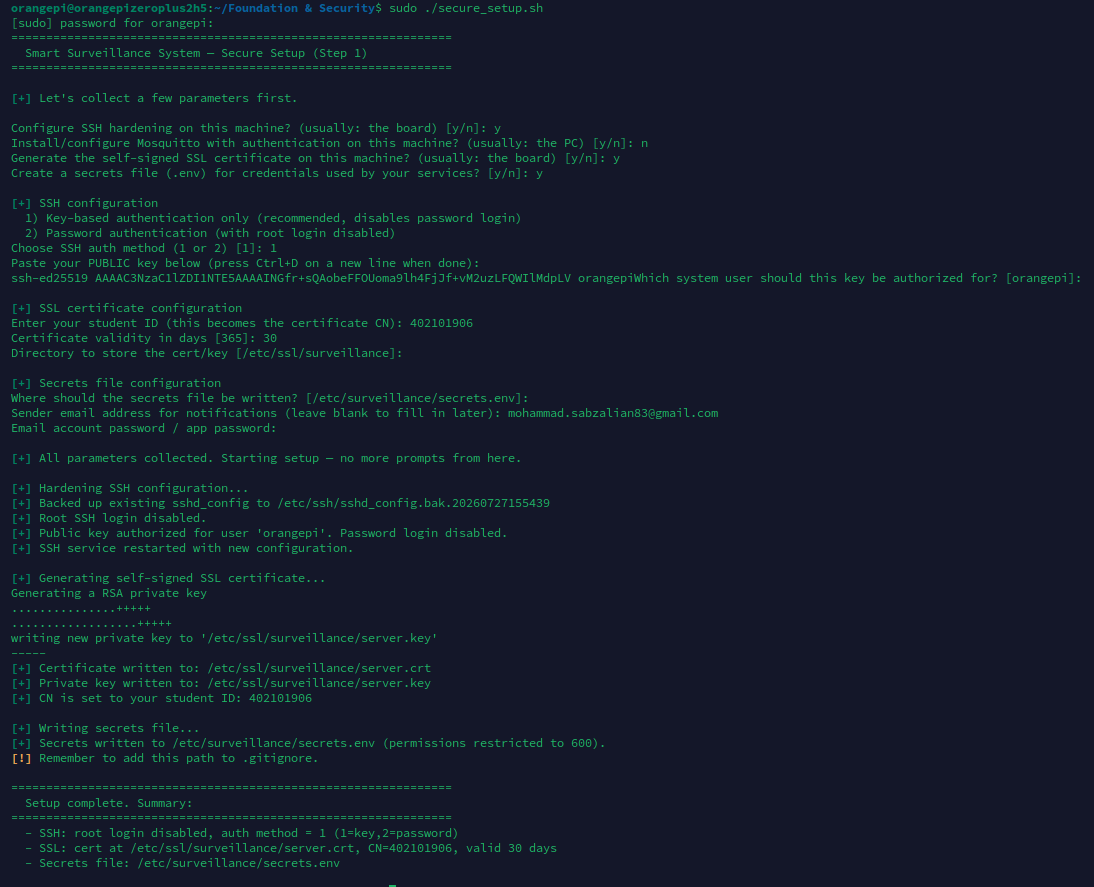
\includegraphics[width=0.85\textwidth]{../../1.Foundation & Security/results/fig/orangepi_setup.png}
\caption{\texttt{secure\_setup.sh} running on the Orange Pi board: SSH key-based hardening and self-signed certificate generation, CN set to the student ID.}\label{fig:orangepi-setup}
\end{figure}

\smartsubsubsection{Deployment on the laptop (MQTT broker host)}

On the laptop, the same script was run with the opposite set of choices:
Mosquitto was installed and configured with a dedicated user
(\texttt{PC\_client}) and anonymous access disabled, while SSH hardening
and certificate generation were skipped, since the laptop is not part of
the board's attack surface for this project.

\begin{figure}[H]
\centering
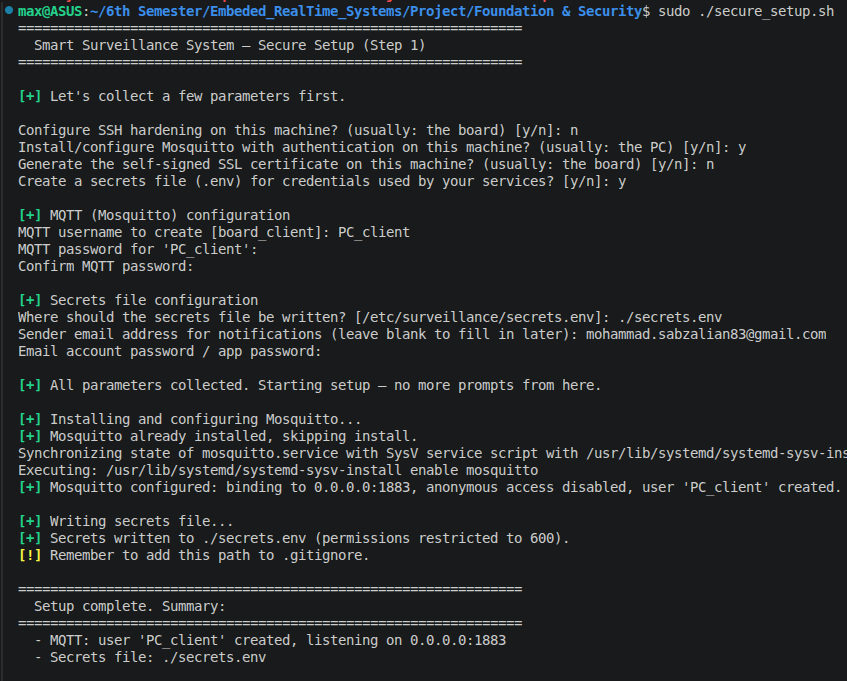
\includegraphics[width=0.85\textwidth]{../../1.Foundation & Security/results/fig/client_setup.png}
\caption{\texttt{secure\_setup.sh} running on the laptop: Mosquitto broker installed and configured with authentication, anonymous access disabled.}\label{fig:client-setup}
\end{figure}

\smartsubsection{Secrets Management}

Both machines end up with a \texttt{secrets.env} file containing the
credentials generated during setup (MQTT username/password, notification
e-mail address), written with file permissions restricted to the owning
user (\highlight{mode 600}). Figures~\ref{fig:orangepi-secret}
and~\ref{fig:client-secret} demonstrate that an unprivileged read of the
file is rejected (\texttt{Permission denied}), and that its contents are
only visible via \texttt{sudo}.

\begin{figure}[H]
\centering
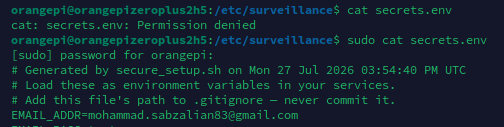
\includegraphics[width=0.85\textwidth]{../../1.Foundation & Security/results/fig/orangepi_secret.png}
\caption{\texttt{secrets.env} on the Orange Pi board: unprivileged read denied, root-privileged read shows the generated credentials.}\label{fig:orangepi-secret}
\end{figure}

\begin{figure}[H]
\centering
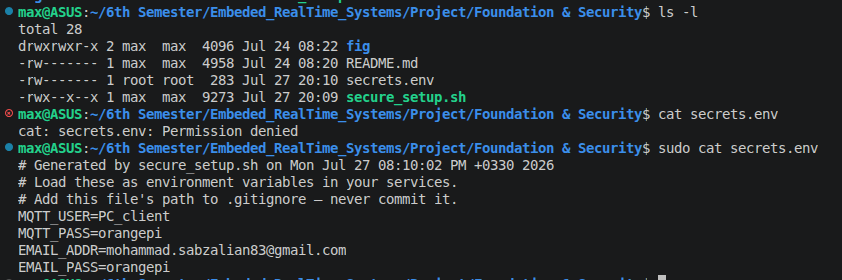
\includegraphics[width=0.85\textwidth]{../../1.Foundation & Security/results/fig/client_secret.png}
\caption{\texttt{secrets.env} on the laptop: directory listing shows \texttt{secure\_setup.sh} is world-executable but the secrets file itself is owner-only (mode 600), matching the board-side result.}\label{fig:client-secret}
\end{figure}

\begin{resultbox}{Secrets policy}
    No credential used anywhere in the Smart Surveillance System — the
    MQTT password, the notification e-mail password, or the TLS private
    key — is ever written into a source file, a systemd unit, or a
    configuration file tracked by version control. Every consumer reads
    these values from \texttt{secrets.env} or the certificate files
    generated by \texttt{secure\_setup.sh} at deploy time.
\end{resultbox}

\smartsubsection{Experiment 3-6: Unauthorized MQTT Login}

With anonymous access disabled on the broker, three deliberately invalid
connection attempts were made from the board using
\texttt{mosquitto\_sub}: no credentials at all, a valid username with an
incorrect password, and an incorrect username with an arbitrary password.
All three were rejected by the broker with an identical
\alert{\texttt{Connection Refused: not authorised}} error, confirming that
credential validation — not merely credential \emph{presence} — is
enforced. A fourth attempt using the correct \texttt{PC\_client} username
and password is shown initiated at the bottom of the same terminal
session.

\begin{figure}[H]
\centering
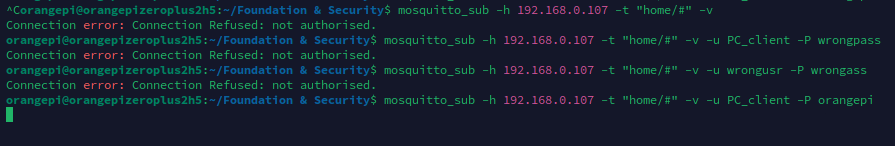
\includegraphics[width=0.95\textwidth]{../../1.Foundation & Security/results/fig/mqtt_test.png}
\caption{Experiment 3-6: three unauthorized MQTT connection attempts (no credentials, wrong password, wrong username), each rejected with \texttt{not authorised}.}\label{fig:mqtt-test}
\end{figure}

\smartsubsection{Experiment 3-7: Unauthorized SSH Login}

Figure~\ref{fig:ssh-test} shows three SSH attempts against the board from
the laptop. The first, a plain \texttt{ssh root@192.168.0.170} with no
identity supplied, is rejected (\texttt{Permission denied (publickey)}) —
expected, since password authentication is disabled entirely. The second
attempt supplies the \emph{correct} private key but still targets the
\texttt{root} account, and is rejected identically: this is the important
result, since it demonstrates that \punder{root login is refused
regardless of key validity}, not merely because the wrong key was used.
The third attempt, using the same key against the intended
\texttt{orangepi} account, succeeds and drops into an authenticated shell.

\begin{figure}[H]
\centering
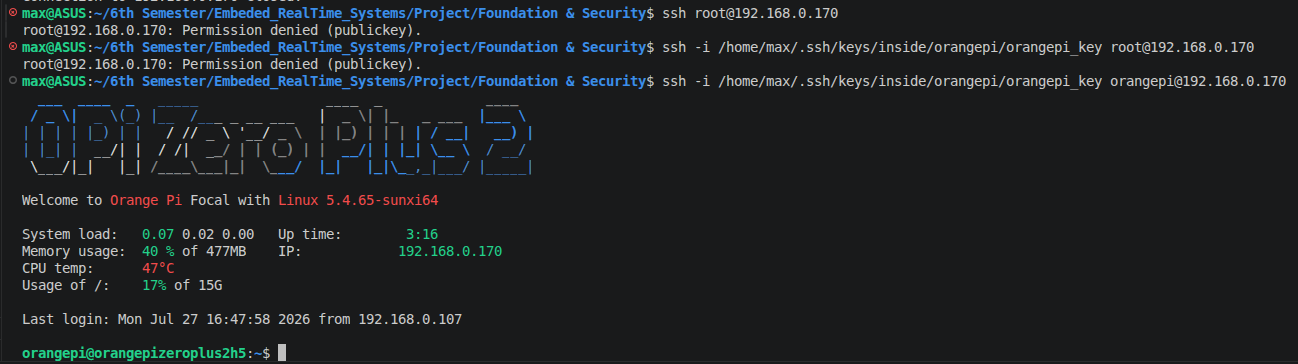
\includegraphics[width=0.95\textwidth]{../../1.Foundation & Security/results/fig/ssh_test.png}
\caption{Experiment 3-7: root SSH login refused both with no key and with a valid key (top two attempts); the same key succeeds against the non-root \texttt{orangepi} account (bottom).}\label{fig:ssh-test}
\end{figure}

\smartsubsection{Certificate Overview}

The generated self-signed certificate and its private key are shown in
Figure~\ref{fig:orangepi-ssl}, confirming the Common Name field is set to
the student ID as required. \alert{This figure has been redacted before
any public distribution of this repository, since it exposes the raw
private key material — see the note in
Section~\ref{sec:foundation-security-notes}.}

\begin{figure}[H]
\centering
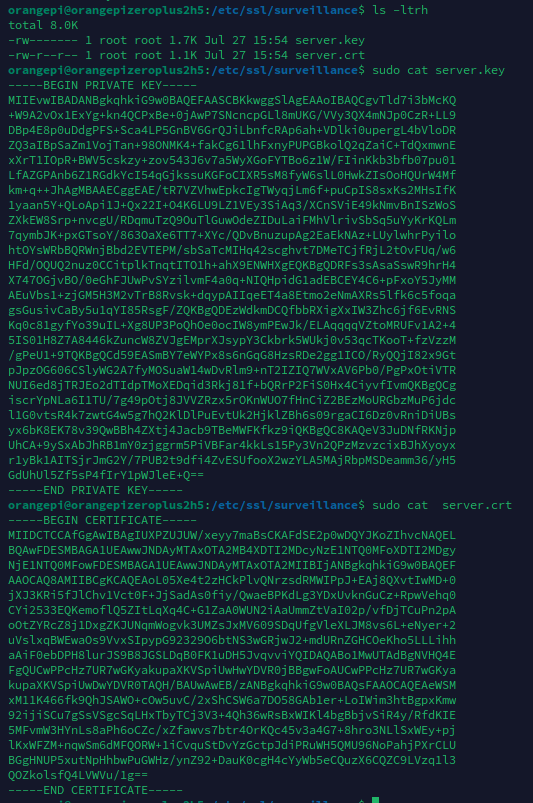
\includegraphics[width=0.85\textwidth]{../../1.Foundation & Security/results/fig/orangepi_ssl.png}
\caption{Self-signed certificate and private key on the board, CN=402101906. Retained for grading purposes only; redacted prior to any public release.}\label{fig:orangepi-ssl}
\end{figure}

\smartsubsection{Notes on This Section's Figures}
\label{sec:foundation-security-notes}

Two figures in this section (Figures~\ref{fig:orangepi-ssl}
and~\ref{fig:client-secret}) show raw credential material — the TLS
private key and the MQTT/e-mail passwords, respectively — captured from a
board that was deployed on a private, NAT-isolated network with no
external exposure. They are retained here for grading transparency but are
\alert{excluded from any public copy of this repository}, consistent with
the same policy already applied to the face-identifying figures in
Section~\ref{sec:image-processing}.

\smartsubsection{Section Summary}

\begin{table}[H]
\centering
\caption{Security controls implemented in this section, mapped to the assignment's baseline requirements.}
\label{tab:security-summary}
\begin{tabular}{ll}
\toprule
\textbf{Control} & \textbf{Status} \\ 
\midrule
Root SSH login & Disabled (both auth methods) \\ 
SSH authentication method & Key-based (board), configurable per-machine \\
MQTT anonymous access & Disabled; dedicated authenticated user \\ 
TLS certificate CN & Student ID (\texttt{402101906}) \\ 
Hardcoded credentials in source & None — all via \texttt{secrets.env} \\ 
Secrets file permissions & \texttt{600} (owner read/write only) \\ 
\bottomrule
\end{tabular}
\end{table}
